%!TEX program = xelatex

\documentclass[compress]{beamer}
%--------------------------------------------------------------------------
% Common packages
%--------------------------------------------------------------------------
\usepackage[english]{babel}
\usepackage{pgfpages} % required for notes on second screen
\usepackage{graphicx}

\usepackage{multicol}

\usepackage{tabularx,ragged2e}
\usepackage{booktabs}

\usepackage{listings}
\lstset{ %
language=[LaTeX]TeX,
basicstyle=\normalsize\ttfamily,
keywordstyle=,
numbers=left,
numberstyle=\tiny\ttfamily,
stepnumber=1,
showspaces=false,
showstringspaces=false,
showtabs=false,
breaklines=true,
frame=tb,
framerule=0.5pt,
tabsize=4,
framexleftmargin=0.5em,
framexrightmargin=0.5em,
xleftmargin=0.5em,
xrightmargin=0.5em
}


%--------------------------------------------------------------------------
% Load theme
%--------------------------------------------------------------------------
\usetheme{hri}

\usepackage{dtklogos} % must be loaded after theme
\usepackage{tikz}
\usetikzlibrary{mindmap,backgrounds,positioning}

%--------------------------------------------------------------------------
% General presentation settings
%--------------------------------------------------------------------------
\title{HRI Beamer Theme}
\subtitle{Demo Presentation}
\date{\today}
\author{Séverin Lemaignan}
\institute{Computer-Human Interaction\\for Learning and Instruction {\Medium
EPFL}}

%--------------------------------------------------------------------------
% Notes settings
%--------------------------------------------------------------------------
%\setbeameroption{show notes on second screen}

\begin{document}
%--------------------------------------------------------------------------
% Titlepage
%--------------------------------------------------------------------------

\maketitle

%\begin{frame}[plain]
%	\titlepage
%\end{frame}

%--------------------------------------------------------------------------
% Table of contents
%--------------------------------------------------------------------------
\section*{Overview}
\begin{frame}{Overview}
	% hideallsubsections ist empfehlenswert für längere Präsentationen
	\tableofcontents[hideallsubsections]
\end{frame}

%--------------------------------------------------------------------------
% Content
%--------------------------------------------------------------------------
\section{Introduction}

\begin{frame}{Theme options}
\begin{table}[]
	\begin{tabularx}{\linewidth}{l>{\raggedright}X}
		\toprule
		\textbf{Option}			& \textbf{Effect} \tabularnewline
		\midrule
		\texttt{noflama}		& Use Arial instead of Flama \tabularnewline
		\texttt{noserifmath}		& Math formula typeset in sans-serif \tabularnewline
		\texttt{nosectionpages} & No inter-section pages \tabularnewline
		\bottomrule
	\end{tabularx}
	\label{tab:options}
\end{table}
\end{frame}

\begin{frame}{Colors 1/2}									

\begin{multicols}{2}

\setbeamercolor{hriRedDemo}{fg=hriRed,bg=white}
\begin{beamercolorbox}[wd=\linewidth,ht=2ex,dp=0.7ex]{hriRedDemo}
	\texttt{hriRed}
\end{beamercolorbox}
\setbeamercolor{hriRedDarkDemo}{fg=hriRedDark,bg=white}
\begin{beamercolorbox}[wd=\linewidth,ht=2ex,dp=0.7ex]{hriRedDarkDemo}
	\texttt{hriRedDark}
\end{beamercolorbox}
\setbeamercolor{hriWarmGreyDarkDemo}{fg=hriWarmGreyDark,bg=white}
\begin{beamercolorbox}[wd=\linewidth,ht=2ex,dp=0.7ex]{hriWarmGreyDarkDemo}
	\texttt{hriWarmGreyDark}
\end{beamercolorbox}
\setbeamercolor{hriWarmGreyLightDemo}{fg=hriWarmGreyLight,bg=white}
\begin{beamercolorbox}[wd=\linewidth,ht=2ex,dp=0.7ex]{hriWarmGreyLightDemo}
	\texttt{hriWarmGreyLight}
\end{beamercolorbox}

\setbeamercolor{hriRedDemoBg}{fg=white,bg=hriRed}
\begin{beamercolorbox}[wd=\linewidth,ht=2ex,leftskip=.5ex,dp=0.7ex]{hriRedDemoBg}
	\texttt{hriRed}
\end{beamercolorbox}
\setbeamercolor{hriRedDarkDemoBg}{fg=white,bg=hriRedDark}
\begin{beamercolorbox}[wd=\linewidth,ht=2ex,leftskip=.5ex,dp=0.7ex]{hriRedDarkDemoBg}
	\texttt{hriRedDark}
\end{beamercolorbox}
\setbeamercolor{hriWarmGreyDarkDemo}{fg=white,bg=hriWarmGreyDark}
\begin{beamercolorbox}[wd=\linewidth,ht=2ex,leftskip=.5ex,dp=0.7ex]{hriWarmGreyDarkDemo}
	\texttt{hriWarmGreyDark}
\end{beamercolorbox}
\setbeamercolor{hriWarmGreyLightDemo}{fg=white,bg=hriWarmGreyLight}
\begin{beamercolorbox}[wd=\linewidth,ht=2ex,leftskip=.5ex,dp=0.7ex]{hriWarmGreyLightDemo}
	\texttt{hriWarmGreyLight}
\end{beamercolorbox}

\end{multicols}

\end{frame}

\begin{frame}{Colors 2/2}
\begin{multicols}{2}

\setbeamercolor{hriSec1Demo}{fg=hriSec1,bg=white}
\begin{beamercolorbox}[wd=\linewidth,ht=2ex,dp=0.7ex]{hriSec1Demo}
	\texttt{hriSec1}
\end{beamercolorbox}
\setbeamercolor{hriSec1DarkDemo}{fg=hriSec1Dark,bg=white}
\begin{beamercolorbox}[wd=\linewidth,ht=2ex,dp=0.7ex]{hriSec1DarkDemo}
	\texttt{hriSec1Dark}
\end{beamercolorbox}
\setbeamercolor{hriSec1CompDemo}{fg=hriSec1Comp,bg=white}
\begin{beamercolorbox}[wd=\linewidth,ht=2ex,dp=0.7ex]{hriSec1CompDemo}
	\texttt{hriSec1Comp}
\end{beamercolorbox}
\setbeamercolor{hriSec1CompDarkDemo}{fg=hriSec1CompDark,bg=white}
\begin{beamercolorbox}[wd=\linewidth,ht=2ex,dp=0.7ex]{hriSec1CompDarkDemo}
	\texttt{hriSec1CompDark}
\end{beamercolorbox}

\setbeamercolor{hriSec2Demo}{fg=hriSec2,bg=white}
\begin{beamercolorbox}[wd=\linewidth,ht=2ex,dp=0.7ex]{hriSec2Demo}
	\texttt{hriSec2}
\end{beamercolorbox}
\setbeamercolor{hriSec2DarkDemo}{fg=hriSec2Dark,bg=white}
\begin{beamercolorbox}[wd=\linewidth,ht=2ex,dp=0.7ex]{hriSec2DarkDemo}
	\texttt{hriSec2Dark}
\end{beamercolorbox}
\setbeamercolor{hriSec2CompDemo}{fg=hriSec2Comp,bg=white}
\begin{beamercolorbox}[wd=\linewidth,ht=2ex,dp=0.7ex]{hriSec2CompDemo}
	\texttt{hriSec2Comp}
\end{beamercolorbox}
\setbeamercolor{hriSec2CompDarkDemo}{fg=hriSec2CompDark,bg=white}
\begin{beamercolorbox}[wd=\linewidth,ht=2ex,dp=0.7ex]{hriSec2CompDarkDemo}
	\texttt{hriSec2CompDark}
\end{beamercolorbox}

\setbeamercolor{hriSec3Demo}{fg=hriSec3,bg=white}
\begin{beamercolorbox}[wd=\linewidth,ht=2ex,dp=0.7ex]{hriSec3Demo}
	\texttt{hriSec3}
\end{beamercolorbox}
\setbeamercolor{hriSec3DarkDemo}{fg=hriSec3Dark,bg=white}
\begin{beamercolorbox}[wd=\linewidth,ht=2ex,dp=0.7ex]{hriSec3DarkDemo}
	\texttt{hriSec3Dark}
\end{beamercolorbox}
\setbeamercolor{hriSec3CompDemo}{fg=hriSec3Comp,bg=white}
\begin{beamercolorbox}[wd=\linewidth,ht=2ex,dp=0.7ex]{hriSec3CompDemo}
	\texttt{hriSec3Comp}
\end{beamercolorbox}
\setbeamercolor{hriSec3CompDarkDemo}{fg=hriSec3CompDark,bg=white}
\begin{beamercolorbox}[wd=\linewidth,ht=2ex,dp=0.7ex]{hriSec3CompDarkDemo}
	\texttt{hriSec3CompDark}
\end{beamercolorbox}

\setbeamercolor{hriSec1DemoBg}{fg=white,bg=hriSec1}
\begin{beamercolorbox}[wd=\linewidth,ht=2ex,leftskip=.5ex,dp=0.7ex]{hriSec1DemoBg}
	\texttt{hriSec1}
\end{beamercolorbox}
\setbeamercolor{hriSec1DarkDemoBg}{fg=white,bg=hriSec1Dark}
\begin{beamercolorbox}[wd=\linewidth,ht=2ex,leftskip=.5ex,dp=0.7ex]{hriSec1DarkDemoBg}
	\texttt{hriSec1Dark}
\end{beamercolorbox}
\setbeamercolor{hriSec1CompDemoBg}{fg=white,bg=hriSec1Comp}
\begin{beamercolorbox}[wd=\linewidth,ht=2ex,leftskip=.5ex,dp=0.7ex]{hriSec1CompDemoBg}
	\texttt{hriSec1Comp}
\end{beamercolorbox}
\setbeamercolor{hriSec1CompDarkDemoBg}{fg=white,bg=hriSec1CompDark}
\begin{beamercolorbox}[wd=\linewidth,ht=2ex,leftskip=.5ex,dp=0.7ex]{hriSec1CompDarkDemoBg}
	\texttt{hriSec1CompDark}
\end{beamercolorbox}

\setbeamercolor{hriSec2DemoBg}{fg=white,bg=hriSec2}
\begin{beamercolorbox}[wd=\linewidth,ht=2ex,leftskip=.5ex,dp=0.7ex]{hriSec2DemoBg}
	\texttt{hriSec2}
\end{beamercolorbox}
\setbeamercolor{hriSec2DarkDemoBg}{fg=white,bg=hriSec2Dark}
\begin{beamercolorbox}[wd=\linewidth,ht=2ex,leftskip=.5ex,dp=0.7ex]{hriSec2DarkDemoBg}
	\texttt{hriSec2Dark}
\end{beamercolorbox}
\setbeamercolor{hriSec2CompDemoBg}{fg=white,bg=hriSec2Comp}
\begin{beamercolorbox}[wd=\linewidth,ht=2ex,leftskip=.5ex,dp=0.7ex]{hriSec2CompDemoBg}
	\texttt{hriSec2Comp}
\end{beamercolorbox}
\setbeamercolor{hriSec2CompDarkDemoBg}{fg=white,bg=hriSec2CompDark}
\begin{beamercolorbox}[wd=\linewidth,ht=2ex,leftskip=.5ex,dp=0.7ex]{hriSec2CompDarkDemoBg}
	\texttt{hriSec2CompDark}
\end{beamercolorbox}

\setbeamercolor{hriSec3Demo}{fg=white,bg=hriSec3}
\begin{beamercolorbox}[wd=\linewidth,ht=2ex,leftskip=.5ex,dp=0.7ex]{hriSec3Demo}
	\texttt{hriSec3}
\end{beamercolorbox}
\setbeamercolor{hriSec3DarkDemo}{fg=white,bg=hriSec3Dark}
\begin{beamercolorbox}[wd=\linewidth,ht=2ex,leftskip=.5ex,dp=0.7ex]{hriSec3DarkDemo}
	\texttt{hriSec3Dark}
\end{beamercolorbox}
\setbeamercolor{hriSec3CompDemo}{fg=white,bg=hriSec3Comp}
\begin{beamercolorbox}[wd=\linewidth,ht=2ex,leftskip=.5ex,dp=0.7ex]{hriSec3CompDemo}
	\texttt{hriSec3Comp}
\end{beamercolorbox}
\setbeamercolor{hriSec3CompDarkDemo}{fg=white,bg=hriSec3CompDark}
\begin{beamercolorbox}[wd=\linewidth,ht=2ex,leftskip=.5ex,dp=0.7ex]{hriSec3CompDarkDemo}
	\texttt{hriSec3CompDark}
\end{beamercolorbox}

\end{multicols}
\end{frame}

\begin{frame}[containsverbatim]{Code}

A slide with some code

\begin{lstlisting}
\section{Meine Sektion}
\subsection{Meine Subsektion}
\begin{frame}
\frametitle{Folientitel}
% Folieninhalt
\end{frame}
\end{lstlisting}
\end{frame}


\begin{frame}[containsverbatim]{Blocks}
\begin{alertblock}{Alert block}
	Aaaaaaagh!
\end{alertblock}

\begin{exampleblock}{Example block}
    Ooooohh!
\end{exampleblock}

\begingroup
\setbeamercolor{block title}{bg=hriSec2Dark}
\setbeamercolor{block body}{bg=hriSec2}
\begin{block}{Block with custom color}
    Oulala!
\end{block}
\endgroup
\end{frame}

\section{Content Examples}

\subsection{Images 1/2}
\begin{frame}{Picture with credit line}
	\begin{figure}
		\centering
        \includegraphicscopyright[width=\linewidth]{photo.jpg}{Copyright EPFL
        2014}
	\end{figure}
\end{frame}

\subsection{Images 2/2}
{
\fullbackground{photo-fullscreen.jpg}
\begin{frame}{Fullscreen picture/graphic}
    \textcolor{white}{
    Normal text goes here.
    }
    \begin{block}{Block with tile}
        \begin{itemize}
            \item Item 1
            \item Item 2
        \end{itemize}
    \end{block}
\end{frame}
}

\imageframe[Children playing with\\the Ranger robot]{photo-fullscreen.jpg}

\subsection{Plotting}
\begin{frame}{Plot with caption}
	\begin{figure}
		\centering
		% GNUPLOT: LaTeX picture with Postscript
\begingroup
  \makeatletter
  \providecommand\color[2][]{%
    \GenericError{(gnuplot) \space\space\space\@spaces}{%
      Package color not loaded in conjunction with
      terminal option `colourtext'%
    }{See the gnuplot documentation for explanation.%
    }{Either use 'blacktext' in gnuplot or load the package
      color.sty in LaTeX.}%
    \renewcommand\color[2][]{}%
  }%
  \providecommand\includegraphics[2][]{%
    \GenericError{(gnuplot) \space\space\space\@spaces}{%
      Package graphicx or graphics not loaded%
    }{See the gnuplot documentation for explanation.%
    }{The gnuplot epslatex terminal needs graphicx.sty or graphics.sty.}%
    \renewcommand\includegraphics[2][]{}%
  }%
  \providecommand\rotatebox[2]{#2}%
  \@ifundefined{ifGPcolor}{%
    \newif\ifGPcolor
    \GPcolorfalse
  }{}%
  \@ifundefined{ifGPblacktext}{%
    \newif\ifGPblacktext
    \GPblacktexttrue
  }{}%
  % define a \g@addto@macro without @ in the name:
  \let\gplgaddtomacro\g@addto@macro
  % define empty templates for all commands taking text:
  \gdef\gplbacktext{}%
  \gdef\gplfronttext{}%
  \makeatother
  \ifGPblacktext
    % no textcolor at all
    \def\colorrgb#1{}%
    \def\colorgray#1{}%
  \else
    % gray or color?
    \ifGPcolor
      \def\colorrgb#1{\color[rgb]{#1}}%
      \def\colorgray#1{\color[gray]{#1}}%
      \expandafter\def\csname LTw\endcsname{\color{white}}%
      \expandafter\def\csname LTb\endcsname{\color{black}}%
      \expandafter\def\csname LTa\endcsname{\color{black}}%
      \expandafter\def\csname LT0\endcsname{\color[rgb]{1,0,0}}%
      \expandafter\def\csname LT1\endcsname{\color[rgb]{0,1,0}}%
      \expandafter\def\csname LT2\endcsname{\color[rgb]{0,0,1}}%
      \expandafter\def\csname LT3\endcsname{\color[rgb]{1,0,1}}%
      \expandafter\def\csname LT4\endcsname{\color[rgb]{0,1,1}}%
      \expandafter\def\csname LT5\endcsname{\color[rgb]{1,1,0}}%
      \expandafter\def\csname LT6\endcsname{\color[rgb]{0,0,0}}%
      \expandafter\def\csname LT7\endcsname{\color[rgb]{1,0.3,0}}%
      \expandafter\def\csname LT8\endcsname{\color[rgb]{0.5,0.5,0.5}}%
    \else
      % gray
      \def\colorrgb#1{\color{black}}%
      \def\colorgray#1{\color[gray]{#1}}%
      \expandafter\def\csname LTw\endcsname{\color{white}}%
      \expandafter\def\csname LTb\endcsname{\color{black}}%
      \expandafter\def\csname LTa\endcsname{\color{black}}%
      \expandafter\def\csname LT0\endcsname{\color{black}}%
      \expandafter\def\csname LT1\endcsname{\color{black}}%
      \expandafter\def\csname LT2\endcsname{\color{black}}%
      \expandafter\def\csname LT3\endcsname{\color{black}}%
      \expandafter\def\csname LT4\endcsname{\color{black}}%
      \expandafter\def\csname LT5\endcsname{\color{black}}%
      \expandafter\def\csname LT6\endcsname{\color{black}}%
      \expandafter\def\csname LT7\endcsname{\color{black}}%
      \expandafter\def\csname LT8\endcsname{\color{black}}%
    \fi
  \fi
  \setlength{\unitlength}{0.0500bp}%
  \begin{picture}(4534.00,3400.00)%
    \gplgaddtomacro\gplbacktext{%
      \csname LTb\endcsname%
      \put(946,772){\makebox(0,0)[r]{\strut{}-140}}%
      \csname LTb\endcsname%
      \put(946,1109){\makebox(0,0)[r]{\strut{}-120}}%
      \csname LTb\endcsname%
      \put(946,1447){\makebox(0,0)[r]{\strut{}-100}}%
      \csname LTb\endcsname%
      \put(946,1784){\makebox(0,0)[r]{\strut{}-80}}%
      \csname LTb\endcsname%
      \put(946,2122){\makebox(0,0)[r]{\strut{}-60}}%
      \csname LTb\endcsname%
      \put(946,2460){\makebox(0,0)[r]{\strut{}-40}}%
      \csname LTb\endcsname%
      \put(946,2797){\makebox(0,0)[r]{\strut{}-20}}%
      \csname LTb\endcsname%
      \put(946,3135){\makebox(0,0)[r]{\strut{} 0}}%
      \csname LTb\endcsname%
      \put(1772,484){\makebox(0,0){\strut{} 100}}%
      \csname LTb\endcsname%
      \put(2766,484){\makebox(0,0){\strut{} 1000}}%
      \csname LTb\endcsname%
      \put(3759,484){\makebox(0,0){\strut{} 10000}}%
      \csname LTb\endcsname%
      \put(176,1919){\rotatebox{-270}{\makebox(0,0){\strut{}amplitude (dB)}}}%
      \put(2607,154){\makebox(0,0){\strut{}frequency (Hz)}}%
    }%
    \gplgaddtomacro\gplfronttext{%
    }%
    \gplbacktext
    \put(0,0){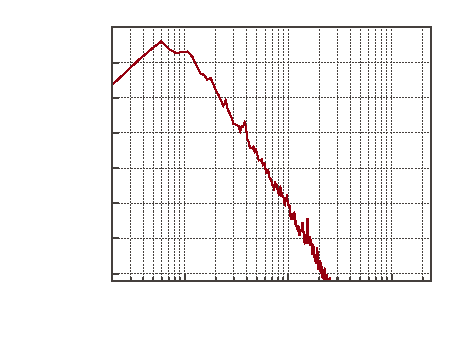
\includegraphics{plot}}%
    \gplfronttext
  \end{picture}%
\endgroup

		\caption{LFE channel frequency spectrum}
	\end{figure}
\end{frame}




\subsection{Table}
\begin{frame}{Table}
\begin{table}[]
	\caption{Selection of window function and their properties}
	\begin{tabular}[]{lrrr}
		\toprule
		\textbf{Window}			& \multicolumn{1}{c}{\textbf{First side lobe}}	
		                    & \multicolumn{1}{c}{\textbf{3\,dB bandwidth}}
		                    & \multicolumn{1}{c}{\textbf{Roll-off}} \\
		\midrule
		Rectangular				& 13.2\,dB	& 0.886\,Hz/bin	& 6\,dB/oct		\\[0.25em]
		Triangular				& 26.4\,dB	& 1.276\,Hz/bin	& 12\,dB/oct	\\[0.25em]
		Hann					& 31.0\,dB	& 1.442\,Hz/bin	& 18\,dB/oct	\\[0.25em]
		Hamming					& 41.0\,dB	& 1.300\,Hz/bin	& 6\,dB/oct		\\
		\bottomrule
	\end{tabular}
	\label{tab:WindowFunctions}
\end{table}
\end{frame}

\subsection{Maths}
\begin{frame}{Maths}
\begin{block}{Fourier Integral}
\begin{equation*}
F(\textrm{j}\omega) = \int\limits_{-\infty}^{\infty} f(t)\cdot\textrm{e}^{-\textrm{j}\omega t} dt
\end{equation*}
\end{block}
\begin{block}{Factorial}
\begin{equation*}
	n! = 1\cdot 2 \cdot 3 \cdot\ldots\cdot n = \prod_{k=1}^n k
\end{equation*}
\end{block}
\end{frame}

\subsection{TikZ 1/2}
\begin{frame}{TikZ figure}
	\begin{figure}
		\centering

\resizebox{\paperwidth}{!}{%

\tikzset{subpart/.style={draw, font=\scriptsize, fill opacity=0.5, text opacity=1, fill=white!50}}

\begin{tikzpicture}[
    >=latex,
    every edge/.style={draw, very thick},
    skill/.style={draw, rounded corners, align=center, inner sep=5pt, fill=black!20},
    label/.style={midway, align=center, font=\scriptsize, fill=white}]

  %%% ORO
    \node at (0,0)[skill, ultra thick, fill=hriSec2Dark!50] (oro) {{\sc Oro} -- Symbolic facts \\ and beliefs management};
  
  %%% HATP
  \node at (-6, 2.5)[skill, fill=hriSec1!50] (hatp) {HATP -- Human-aware \\ symbolic task planning};
  
  %%% DIALOGS
  \node at (-6, -3) [skill, fill=hriSec3Dark!50] (dialogs) {{\sc Dialogs} \\ Dialogue processing};

  %%% SPARK
  \node at (4,-3.5)[skill, fill=hriSec3!50] (spark) {%
      \begin{tikzpicture}
          \node at (0,0) (geom) {{\sc Spark} -- Geometric \& Temporal Reasoning};
        \node [subpart, below=0.2 of geom.south west, anchor=north west] (world-update) {Sensors fusion};
        \node [subpart, right=0.2 of world-update] (geom-model) {Geometric model of the environment};
        \node [subpart, right=0.2 of geom-model] (fact-prod) {Symbolic facts production};
      \end{tikzpicture}
    };

  %%% MHP
    \node at (9,0)[skill, fill=hriSec3CompDark!50] (mhp) {{\sc mhp} -- Human-aware \\ Motion and Manipulation \\ Planning};

  %%% SHARY
  \node at (4,4.5)[skill, fill=hriSec1Comp!50] (shary) {%
      \begin{tikzpicture}
        \node at (0,0) (exec) {Execution Controller};
        \node [subpart, below=0.2 of exec.south west, anchor=north west] (plans) {Goal \& Plans \\ management};
        \node [subpart, right=0.2 of plans] (sit-asses) {Situation assessment \\ and context management};
        \node [subpart, right=0.2 of sit-asses] {Action instantiation, \\ execution and monitoring};
      \end{tikzpicture}
    };


  %%% LOWLEVEL
  \node [skill, below=0.7 of spark] (lowlevel) {%
      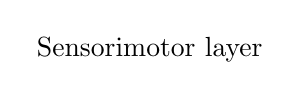
\begin{tikzpicture}
        \node at (0,0) (sensori) {Sensorimotor layer};
        %\node [subpart, below=0.2 of sensori.south west, anchor=north west, align=left] (perception) {{\bf Perception} \\ 2D markers, RGB-D, motion capture};
        %\node [subpart, align=right, right=0.2 of perception] {{\bf Actuation} \\ Head's pan-tilt unit, grippers, arms, wheels};
      \end{tikzpicture}
  };

  %%% Separation between deliberative layer and sensori-motor layer
  \draw[dotted, thick] (-8,-5) -- (12, -5);

  %%% Relations between components
  \path (shary.340) edge [<->, bend left] node[label] {motion plan \\ requests} (mhp);
  \path (shary.west) edge [<->, bend right] node[label] {shared \\ plans} (hatp);
  \path (hatp) edge [<->, bend right] node[label] {world model and \\ agents beliefs} (oro.170);
  \path (dialogs) edge [<->, bend left] node[label] {natural language \\ grounding} (oro.190);
  \path (spark.100) edge [->, bend right] node[label] {symbolic \\ facts} (oro);
  \path (spark.5) edge [->, bend right] node[label] {environment\\model} (mhp);
  \path (shary) edge [<->, bend left] node[label] {events, \\ world model and \\ agents beliefs} (oro);
  \path (shary) edge [<->, bend left] node[label] {action monitoring \\ and management of \\ position hypotheses} (spark);
  \path (lowlevel) edge [->] (spark);
  \path (lowlevel.east) edge [<-, bend right=80, looseness=1.5] node[label] {atomic\\actions} (shary.east);

\end{tikzpicture}
}
	\end{figure}
\end{frame}


\subsection{TikZ 2/2}

\begin{frame}{Mindmap with TikZ}
\centering
\begin{tikzpicture}[scale=0.88]
	%\tikzset{every child/.append style={level distance=250}}
	\path[mindmap,concept color=hriWarmGreyLight,text=hriWarmGreyDark]
	node[concept] {\TeX}
	[clockwise from=-30]
	child[concept color=hriSec2Dark,text=white] { node[concept] {\textcolor{white}{\XeTeX}} }
	child[concept color=hriSec1CompDark,text=white] { node[concept] {\ConTeXt} }
	child[concept color=hriSec1Dark,text=white] { node[concept] {\LaTeX} };
\end{tikzpicture}
\end{frame}

\subsection{Video clips}

\begin{frame}{Video clip}
    \centering
    \video{7cm}{videoclip.webm}

    The video is not directly embedded in the PDF file: you need to copy it next
    to your PDF.

\end{frame}

\videoframe{videoclip.webm}


\subsection{References on page}

{
    \paper{G\"odel et al., {\Medium Life is incomplete}, 1923}

    \begin{frame}{Litterature reference}
        You can add a reference to a paper in the page footer.
    \end{frame}
}



\subsection{Footnotes}
\begin{frame}{Footnotes}
Lorem ipsum dolor sit amet, consetetur sadipscing elitr, sed diam nonumy
eirmod tempor invidunt ut labore et dolore magna aliquyam erat, sed diam
voluptua. At vero eos et accusam et justo duo dolores et ea rebum. Stet
clita kasd gubergren, no sea takimata sanctus est Lorem ipsum dolor sit
amet. Lorem \footnote{Lorem ipsum dolor sit amet} ipsum dolor sit amet,
consetetur sadipscing elitr, sed diam nonumy eirmod tempor invidunt ut
labore et dolore magna aliquyam erat, sed diam voluptua. At vero eos et
accusam et justo duo dolores et ea rebum. Stet clita kasd gubergren, no sea
takimata sanctus est Lorem ipsum dolor sit amet.

\end{frame}

\subsection{Columns}
\begin{frame}{Two Columns}
    \begin{multicols}{2}
        Lorem ipsum dolor sit amet, consetetur sadipscing elitr, sed diam nonumy eirmod tempor invidunt ut labore et dolore magna aliquyam erat, sed diam voluptua. At vero eos et accusam et justo duo dolores et ea rebum. Stet clita kasd gubergren, no sea takimata sanctus est Lorem ipsum dolor sit amet.
        \begin{itemize}
            \item item
            \item item
        \end{itemize}
    \end{multicols}
\end{frame}

\begin{frame}{Bibliography}
	\begin{thebibliography}{10}
    
	\beamertemplatebookbibitems
	\bibitem{Oppenheim2009}
	Alan~V.~Oppenheim
	\newblock \doublequoted{Discrete-Time Signal Processing}
	\newblock Prentice Hall Press, 2009

	\beamertemplatearticlebibitems
	\bibitem{EBU2011}
	European~Broadcasting~Union
	\newblock \doublequoted{Specification of the Broadcast Wave Format (BWF)}
	\newblock 2011
  \end{thebibliography}
\end{frame}

\end{document}






